\documentclass{article}

\PassOptionsToPackage{numbers,sort&compress}{natbib}
\usepackage[preprint]{neurips_2021}

\usepackage[utf8]{inputenc}
\usepackage[T1]{fontenc}
\usepackage{hyperref}
\usepackage{url}
\usepackage{booktabs}
\usepackage{amsfonts}
\usepackage{nicefrac}
\usepackage{microtype}
\usepackage{xcolor}
\usepackage{graphicx}
\usepackage{subcaption}
\usepackage{multirow}
\usepackage{array}
\usepackage{float}
\usepackage{adjustbox}
\usepackage{amsthm}
\usepackage{amsmath}
\usepackage{amssymb}
\usepackage{mathtools}
\usepackage{enumitem}
\usepackage{algorithm}
\usepackage{algpseudocode}

\title{STAWA-Old: Domain Generalization by Seeking Functional Stationarity}

\author{Anonymous Authors}

\newtheorem{theorem}{Theorem}
\newtheorem{proposition}{Proposition}
\newtheorem{lemma}{Lemma}
\newtheorem{corollary}{Corollary}
\newtheorem{definition}{Definition}
\newtheorem{assumption}{Assumption}
\newtheorem{remark}{Remark}

\newcommand{\RR}{\mathbb{R}}
\newcommand{\EE}{\mathbb{E}}
\newcommand{\tr}{\operatorname{tr}}
\newcommand{\argmin}{\operatorname*{arg\,min}}
\newcommand{\diag}{\operatorname{diag}}
\newcommand{\TBD}{\textbf{TBD}}
\newcommand{\etal}{\textit{et al.}}
\newcommand{\ie}{\textit{i.e.}}
\newcommand{\eg}{\textit{e.g.}}
\newcommand{\iid}{i.i.d.}
\newcommand{\ood}{OOD}
\newcommand{\iidcaps}{IID}
\newcommand{\stawa}{\textup{\textsc{STAWA}}}
\newcommand{\swad}{\textup{\textsc{SWAD}}}
\newcommand{\riwa}{\textup{\textsc{RIWA}}}
\newcommand{\TV}{\operatorname{TV}}
\newcommand{\diam}{\operatorname{diam}}
\newcommand{\norm}[1]{\left\lVert #1 \right\rVert}
\newcommand{\inner}[2]{\left\langle #1, #2 \right\rangle}

\begin{document}

\maketitle

\begin{abstract}
This manuscript records the original \textbf{STAWA-Old} formulation that preceded the plateau-constrained STAWA-New revision. Single-run post-hoc methods matter in domain generalization because they can be attached to strong empirical risk minimization pipelines without retraining. The canonical method in this regime is \swad, which selects and averages dense checkpoints by seeking flat minima in parameter space. We argue that flatness is only an indirect proxy for the label-free domain generalization problem. The original Stationarity-Aware Weight Averaging (\stawa) scores every checkpoint globally by source validation loss plus the mean and spread of short-horizon predictive drift on a held-out support set. We show that functional drift controls the distance from a checkpoint to its local prediction plateau, that the drift mean and variance together upper-bound hidden unstable subsets and density-ratio shifts, and that the empirical \stawa{} components concentrate uniformly over dense checkpoint sequences. We then derive a target-risk certificate whose controllable terms are validation fit, mean drift, and drift variance, and prove a constructive separation theorem: there exist checkpoints with identical validation loss and identical local flatness statistics that any flatness-only selector treats as equivalent, while \stawa{} strictly prefers the checkpoint with lower target risk. Finally, we justify dense checkpointing and contiguous low-score window averaging under local regularity assumptions. This archival manuscript is preserved so that STAWA-Old and STAWA-New can be compared directly under the same replay protocol; all new \stawa{} quantitative results remain intentionally marked as \TBD{} pending execution.
\end{abstract}

\section{Introduction}

Domain generalization (DG) asks for a model that performs well on an unseen target environment using only source data at training time. The methods that have mattered most in practice are often the ones that preserve an ordinary training pipeline and add a simple post-hoc model-selection rule. \swad{} \citep{cha2021wad} is the reference point in this regime. It is single-run, post-hoc, and empirically strong: on the five standard DomainBed benchmarks with ResNet-50, \swad{} reports an average accuracy of $66.9$, improving over ERM's $63.3$ and over the best previous competitor's $65.3$ in the same evaluation family \citep{cha2021wad}. Diverse Weight Averaging (DiWA) later showed that weight averaging can go higher, up to $68.0$, but its strongest setting relies on many models or many runs \citep{rame2022diwa}.

The practical question is therefore narrow:
\begin{quote}
Can a single training trajectory support a post-hoc selector that is as simple as \swad{}, requires no domain labels, and targets domain shift more directly than pooled flatness?
\end{quote}

Our answer is \stawa{}, Stationarity-Aware Weight Averaging. In this original formulation, the principle is:
\begin{quote}
    Checkpoints with low validation loss and low future predictive drift are better candidates for robust post-hoc averaging under shift.
\end{quote}
Instead of probing the loss landscape in parameter space, \stawa{} probes the trajectory in \emph{function space}. At checkpoint $\theta_t$, it measures how much the predictions of $\theta_t$ change over the next $H$ checkpoints on a held-out support set, forms a global composite score from source validation loss plus drift statistics, and then averages a contiguous low-score window around the best checkpoint. The method is intentionally retrospective: it is designed to evaluate checkpoints inside one completed trajectory, not to serve as an online stopping rule.

This move is conceptually simple but theoretically nontrivial. Generalization theory for learning algorithms that do not converge shows that stable long-run behavior of the learning dynamics, not literal fixed-point convergence, is the relevant object \citep{chandramoorthy2022nonconvergent}. Checkpoint-ensemble work already showed that a single trajectory contains useful function-level information \citep{chen2017checkpoint}. What is missing is a \emph{domain-generalization checkpoint selector} built on the same dynamical object. That is the role of \stawa{}.

The strongest version of the intuition is not just ``low average drift.'' A checkpoint can have small mean drift while still containing a small pocket of violently unstable examples, and that pocket may be exactly where \ood{} failure lives. \stawa{} therefore uses two function-space statistics:
\begin{itemize}[leftmargin=1.4em]
    \item the mean predictive drift, which measures departure from a local plateau; and
    \item the drift spread, which measures whether a hidden unstable subset is still being renegotiated by SGD.
\end{itemize}

We make five contributions.
\begin{enumerate}[leftmargin=1.4em]
    \item We introduce STAWA-Old, a label-free, single-run post-hoc DG method that ranks checkpoints globally by source validation loss plus mean and spread of short-horizon predictive drift.
    \item We prove that functional drift controls the risk gap between a checkpoint and its local prediction plateau, while mean and variance together control hidden unstable subsets and bounded density-ratio shifts.
    \item We prove uniform concentration of the empirical \stawa{} components over dense checkpoint sequences and derive an explicit target-risk certificate whose controllable terms are validation fit, drift mean, and drift spread.
    \item We prove a constructive separation theorem showing that flatness-only selectors can be provably blind to target-relevant functional instability that \stawa{} detects.
    \item We justify dense checkpoint sampling and low-drift weight averaging under local regularity assumptions, and provide a complete NeurIPS-style manuscript with proofs, figures, protocol, and published baselines; all new \stawa{} result cells remain marked \TBD{}.
\end{enumerate}

\begin{remark}
This paper does \emph{not} claim an unconditional theorem that \stawa{} empirically dominates \swad{}, DiWA, or every other DG method on all tasks. Such a theorem would be indefensible. Our theory instead proves that \stawa{} targets a different object, that this object yields a stronger certificate under explicit assumptions, and that flatness-only selectors provably miss it on a nontrivial class of examples.
\end{remark}

\begin{figure}[t]
    \centering
    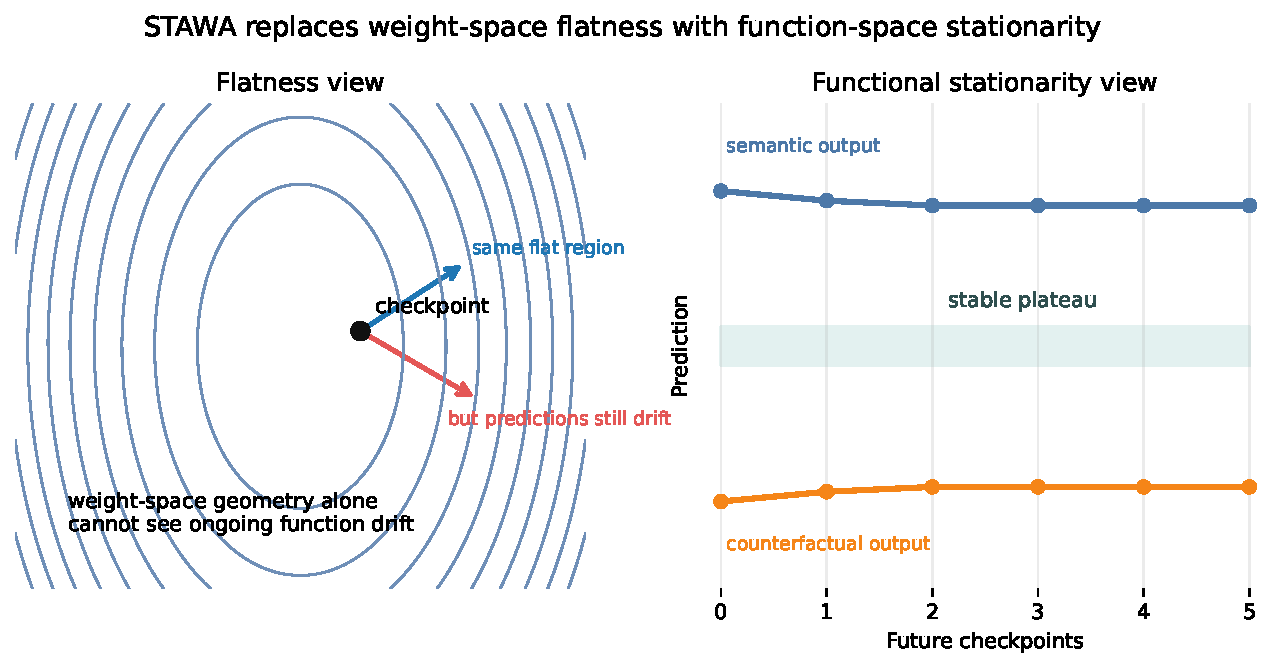
\includegraphics[width=\linewidth]{figures/flatness_vs_stationarity.pdf}
    \caption{\textbf{Conceptual shift from flatness to functional stationarity.} \swad{} probes geometric robustness in weight space. STAWA-Old asks whether the predictor itself is both low-loss and functionally calm under the actual training dynamics. Two checkpoints can have similar validation loss and similar flatness while still differing strongly in future predictive drift.}
    \label{fig:concept}
\end{figure}

\section{Related Work}

\paragraph{Single-run post-hoc DG.}
\swad{} \citep{cha2021wad} is the canonical single-run post-hoc DG method. Its practical appeal comes from dense checkpoints, overfit-aware windowing, and a final weight average. DiWA \citep{rame2022diwa} shows that more diverse averaging can improve \ood{} performance further, but the strongest results rely on many models or runs. \stawa{} stays in the \swad{} regime and changes the selection principle rather than the computational regime.

\paragraph{Weight averaging and mode connectivity.}
SWA \citep{izmailov2018swa}, mode-connectivity work \citep{garipov2018fge,frankle2020linear}, and model soups \citep{wortsman2022soups} established that averaging nearby models can improve generalization when they live in a common low-loss region. \swad{} imports this logic into DG through flatness. \stawa{} keeps the final averaging step but changes the object being measured: not weight-space geometry first, but functional stationarity first.

\paragraph{Stability and non-convergent training.}
Algorithmic stability is a standard route to generalization \citep{bousquet2002stability,hardt2016train}. More recently, \citet{chandramoorthy2022nonconvergent} showed that when learning algorithms do not converge to a fixed point, the relevant object is the stability of their time-asymptotic behavior. \stawa{} converts this qualitative principle into a practical post-hoc selector by estimating local stationarity from dense checkpoints.

\paragraph{Single-run trajectory exploitation.}
Checkpoint ensembles exploit multiple points along one training trajectory to improve performance without retraining \citep{chen2017checkpoint}. \stawa{} differs in a crucial way: it does not use the trajectory only as a source of diverse models to average. It uses the trajectory itself to define a DG-specific selection signal.

\section{Stationarity-Aware Weight Averaging}
\label{sec:method}

Assume a single training run produces checkpoints $\{\theta_t\}_{t=1}^{K}$. For model selection we reserve:
\begin{itemize}[leftmargin=1.4em]
    \item a held-out support set $U = \{x_i\}_{i=1}^{m}$ used to measure short-horizon predictive drift, and
    \item a labeled validation set $V = \{(x_j,y_j)\}_{j=1}^{n}$ used for ordinary checkpoint scoring.
\end{itemize}
Neither set requires domain labels.

Let $p_t(x)$ denote the predictive output of checkpoint $\theta_t$ at input $x$. For classification, $p_t(x)$ is a probability vector in the simplex. For regression, $p_t(x)$ is the predicted value. We assume only that the prediction space is convex and equipped with a norm-induced discrepancy $d$.

\subsection{Short-horizon functional drift}

\begin{definition}[Per-example predictive drift]
Fix a horizon $H \ge 1$. For checkpoint $t$ and example $x$, define
\begin{equation}
    \Delta_t(x)
    \triangleq
    \frac{1}{H}\sum_{h=1}^{H} d\!\left(p_t(x), p_{t+h}(x)\right).
    \label{eq:delta}
\end{equation}
\end{definition}

\paragraph{What ``stationarity'' means in this paper.}
We use the term \emph{functional stationarity} in a local and operational sense: a checkpoint is more stationary when both its average future predictive drift $\mu_t$ and its cross-example drift spread $\sigma_t$ are small over a fixed short horizon. This is weaker than convergence to a fixed point and weaker than claiming invariance. It is a directly measurable local calmness property of the predictor under the realized training dynamics.

\paragraph{Normalization and checkpoint spacing.}
If checkpoints are saved every $q$ optimizer steps, Eq.~\eqref{eq:delta} is already normalized per fixed trajectory interval. When checkpoints are irregularly spaced, let $\tau_t$ denote cumulative optimization time and replace Eq.~\eqref{eq:delta} by the rate-normalized variant
\begin{equation}
    \Delta_t^{\mathrm{rate}}(x)
    \triangleq
    \frac{1}{H}\sum_{h=1}^{H}
    \frac{
        d\!\left(p_t(x), p_{t+h}(x)\right)
    }{
        \tau_{t+h}-\tau_t
    }.
    \label{eq:delta_rate}
\end{equation}
All theory below is written for the fixed-spacing case to keep the notation simple; the normalized form is the practical fallback when checkpoint cadence varies.

The corresponding support-set statistics are
\begin{align}
    \mu_t &\triangleq \frac{1}{m}\sum_{i=1}^{m}\Delta_t(x_i), \label{eq:mu}\\
    \sigma_t^2 &\triangleq \frac{1}{m}\sum_{i=1}^{m}\left(\Delta_t(x_i)-\mu_t\right)^2. \label{eq:sigma}
\end{align}
Here $\mu_t$ measures average departure from a stable functional plateau, while $\sigma_t$ measures whether the remaining drift is concentrated on a hidden subset of examples.

\subsection{Plateau-constrained stationarity score}

Let
\begin{equation}
    L_V(\theta_t)
    \triangleq
    \frac{1}{n}\sum_{j=1}^{n}\ell\!\left(y_j, p_t(x_j)\right)
\end{equation}
be the labeled source-validation loss at checkpoint $t$. The stationarity score is
\begin{equation}
    J_t
    \triangleq
    \lambda_1 \mu_t
    + \lambda_2 \sigma_t,
    \label{eq:stationarity_score}
\end{equation}
where $\lambda_1,\lambda_2 \ge 0$ are hyperparameters.

The simplest mean-only variant sets $\lambda_2=0$. Our default method keeps both terms because the variance term is the easiest rigorous way to control hidden unstable pockets.

\paragraph{Global selector score.}
The original STAWA selector scores the full trajectory with the composite quantity
\begin{equation}
    S_t
    \triangleq
    L_V(\theta_t) + J_t,
    \label{eq:analysis_score}
\end{equation}
and chooses checkpoints directly from this score without a separate loss-admissible gate.

\paragraph{Why future drift is the right post-hoc object.}
The stationarity score is deliberately forward-looking. \stawa{} does not ask whether a checkpoint is already calm in isolation; it asks whether that checkpoint is the entrance to a stable local phase of the completed trajectory. That is a retrospective question, but retrospective selection is exactly the regime in which \swad{} and related post-hoc averaging methods are deployed.

\subsection{Checkpoint selection and averaging}

Let
\begin{equation}
    t^\star \in \argmin_t S_t.
\end{equation}
Define the low-score set
\begin{equation}
    W_{\delta}
    \triangleq
    \left\{
        t : S_t \le S_{t^\star} + \delta
    \right\},
\end{equation}
restricted to the connected component containing $t^\star$. The final model is the weight average
\begin{equation}
    \bar \theta_{\stawa}
    \triangleq
    \sum_{t\in W_{\delta}} w_t \theta_t,
    \qquad
    w_t \ge 0,
    \quad
    \sum_{t\in W_{\delta}} w_t = 1.
\end{equation}
Uniform weights are the default.

\begin{figure*}[t]
    \centering
    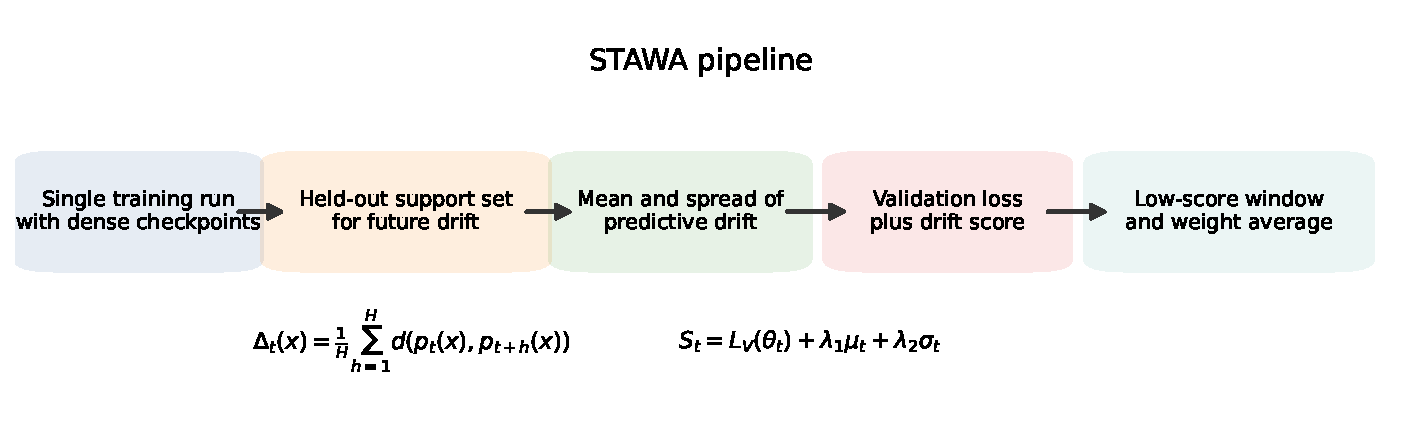
\includegraphics[width=0.96\textwidth]{figures/stawa_pipeline.pdf}
    \caption{\textbf{\stawa{} pipeline.} Starting from a single dense training trajectory, STAWA-Old computes short-horizon predictive drift on a held-out support set, adds it to source validation loss to form a global selector score, and averages a contiguous low-score window around the best checkpoint. No domain labels are needed at any stage.}
    \label{fig:pipeline}
\end{figure*}

\begin{algorithm}[t]
    \caption{\stawa{} (\textsc{Stationarity-Aware Weight Averaging})}
    \label{alg:stawa}
    \begin{algorithmic}[1]
        \Require Checkpoints $\{\theta_t\}_{t=1}^{K}$ from one training run; held-out support set $U$; labeled validation set $V$; horizon $H$; weights $\lambda_1,\lambda_2$; drift width $\delta$
        \For{$t=1,\dots,K-H$}
            \For{each $x_i \in U$}
                \State $\Delta_t(x_i) \gets \frac{1}{H}\sum_{h=1}^{H} d(p_t(x_i), p_{t+h}(x_i))$
            \EndFor
            \State $\mu_t \gets \frac{1}{m}\sum_i \Delta_t(x_i)$
            \State $\sigma_t \gets \sqrt{\frac{1}{m}\sum_i (\Delta_t(x_i)-\mu_t)^2}$
            \State $L_V(\theta_t) \gets \frac{1}{n}\sum_j \ell(y_j, p_t(x_j))$
            \State $J_t \gets \lambda_1 \mu_t + \lambda_2 \sigma_t$
        \EndFor
        \State $S_t \gets L_V(\theta_t) + J_t$
        \State $t^\star \gets \argmin_t S_t$
        \State $W_{\delta} \gets$ connected low-score window around $t^\star$
        \State \Return $\bar \theta_{\stawa} = \sum_{t\in W_{\delta}} w_t \theta_t$
    \end{algorithmic}
\end{algorithm}

\paragraph{Practical complexity.}
The method needs only forward passes on cached checkpoints. For classification, the main practical object is a short-horizon divergence such as total variation, Jensen--Shannon, or KL between predictive distributions. Since the selector is post-hoc and uses only dense checkpoints from one completed run, \stawa{} remains in the same deployment regime as \swad{}.

\section{Theory}
\label{sec:theory}

We now analyze \stawa{} under explicit assumptions. The theory has four parts:
\begin{enumerate}[leftmargin=1.4em]
    \item drift controls the gap to a local prediction plateau,
    \item mean and variance control hidden unstable subsets and density-ratio shifts,
    \item the empirical components and the global selector score concentrate over dense checkpoint sequences,
    \item flatness-only selectors can be blind to the signal \stawa{} measures.
\end{enumerate}

The theory target is deliberately modest. We do not try to prove that low drift universally implies good domain generalization. Instead, we analyze STAWA-Old as a \emph{selector within one trajectory}: does the global score $S_t = L_V(\theta_t) + J_t$ produce a tighter target-risk certificate and a more informative ranking signal than flatness alone?

\subsection{A checkpoint is close to its local plateau when drift is small}

\begin{definition}[Prediction plateau]
For checkpoint $t$, define the horizon-$H$ plateau predictor
\begin{equation}
    \bar p_{t,H}(x)
    \triangleq
    \frac{1}{H+1}\sum_{h=0}^{H} p_{t+h}(x).
    \label{eq:plateau}
\end{equation}
\end{definition}

\begin{assumption}[Convex Lipschitz loss]
\label{ass:lipschitz}
The loss $\ell(y,p)$ is convex in the prediction argument $p$ and $L_d$-Lipschitz with respect to the norm-induced discrepancy $d$:
\begin{equation}
    |\ell(y,p)-\ell(y,q)| \le L_d\, d(p,q)
    \qquad
    \text{for all } y,p,q.
\end{equation}
\end{assumption}

This assumption covers regression with squared loss on bounded outputs and classification with clipped probabilities under the $\ell_1$/TV metric.

\begin{theorem}[Functional drift controls distance to the local plateau]
\label{thm:plateau}
Under Assumption~\ref{ass:lipschitz}, for any data distribution $Q$ over inputs and labels,
\begin{equation}
    R_Q(p_t)
    \le
    R_Q(\bar p_{t,H}) + L_d \mu_t^Q,
    \label{eq:plateau_bound}
\end{equation}
where
\begin{equation}
    \mu_t^Q \triangleq \EE_{x\sim Q_X}\!\left[\Delta_t(x)\right].
\end{equation}
Moreover,
\begin{equation}
    R_Q(\bar p_{t,H})
    \le
    \frac{1}{H+1}\sum_{h=0}^{H} R_Q(p_{t+h}).
    \label{eq:plateau_jensen}
\end{equation}
\end{theorem}

Theorem~\ref{thm:plateau} is the basic stationarity result: if predictive drift is small, the current checkpoint is already close in risk to the local prediction plateau generated by the continued training dynamics.

\subsection{Why the variance term matters}

The next theorem formalizes the ``hidden unstable subset'' intuition.

\begin{theorem}[Hidden unstable subsets are controlled by mean and variance]
\label{thm:subset}
Let $\Delta$ be any square-integrable nonnegative random variable with mean $\mu$ and standard deviation $\sigma$ under a probability distribution $P$. Then for every measurable subset $A$ with $P(A)=\rho \in (0,1]$,
\begin{equation}
    \EE[\Delta \mid A]
    \le
    \mu + \sigma \sqrt{\frac{1-\rho}{\rho}}.
    \label{eq:subset}
\end{equation}
\end{theorem}

Theorem~\ref{thm:subset} explains why mean drift alone is incomplete. A checkpoint can have small average drift while a small target-relevant subset is still highly unstable. The variance term controls precisely this failure mode.

\begin{corollary}[Density-ratio shift bound for target drift]
\label{cor:density}
Let $P_U$ be the support-set marginal and let $P_T$ be a target marginal satisfying
\begin{equation}
    \frac{dP_T}{dP_U}(x) \le \frac{1}{\rho}
    \qquad
    \text{for } P_U\text{-almost every } x
\end{equation}
for some $\rho \in (0,1]$. Then the target drift obeys
\begin{equation}
    \mu_t^T
    \le
    \mu_t^U + \sigma_t^U \sqrt{\frac{1-\rho}{\rho}},
    \label{eq:density_bound}
\end{equation}
where $\mu_t^U,\sigma_t^U$ are the mean and standard deviation of $\Delta_t(x)$ under $P_U$.
\end{corollary}

Corollary~\ref{cor:density} is the key DG interpretation: if the target environment is a bounded density-ratio reweighting of the support family, then the mean and spread of support drift directly control target drift.

\begin{figure}[t]
    \centering
    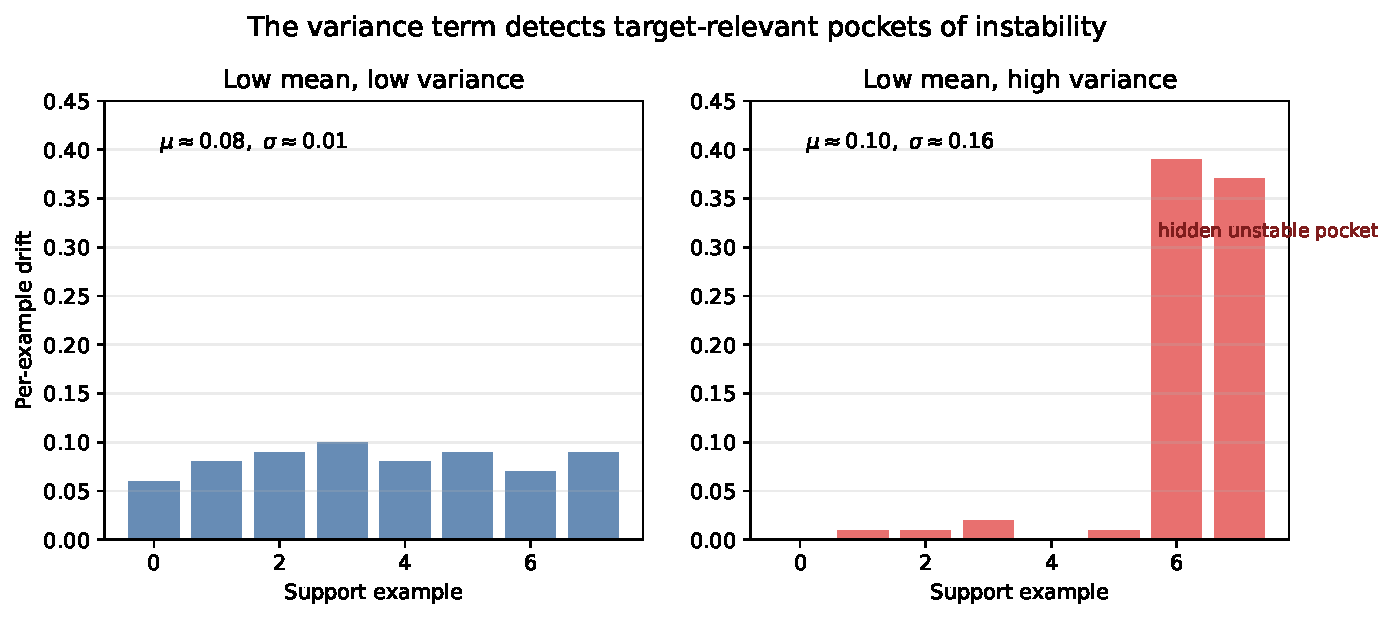
\includegraphics[width=\linewidth]{figures/mean_variance_hidden_subset.pdf}
    \caption{\textbf{Why variance matters.} Two checkpoints can have similar mean drift but very different drift concentration across examples. The variance term penalizes hidden unstable pockets, which are the natural place for \ood{} failure to hide.}
    \label{fig:subset}
\end{figure}

\subsection{Empirical component concentration and plateau recovery}

The method uses empirical support and validation sets, so both the loss plateau and the stationarity ranking must be statistically stable.

\begin{proposition}[Uniform concentration of empirical validation loss and stationarity score]
\label{prop:concentration}
Assume $0 \le \ell \le 1$ and $0 \le d \le 1$. Let $\hat \mu_t,\hat \sigma_t,\hat L_V(\theta_t)$ be the empirical quantities computed from support size $m$ and validation size $n$. Define the population stationarity score
\begin{equation}
    J_t^\star
    \triangleq
    \lambda_1 \mu_t^U + \lambda_2 \sigma_t^U,
\end{equation}
and its empirical counterpart
\begin{equation}
    \hat J_t \triangleq \lambda_1 \hat \mu_t + \lambda_2 \hat \sigma_t.
\end{equation}
Then with probability at least $1-\delta$, simultaneously for all $t=1,\dots,K-H$,
\begin{equation}
    \left| \hat L_V(\theta_t) - R_V(p_t) \right|
    \le
    \sqrt{\frac{\log(4(K-H)/\delta)}{2n}},
    \label{eq:conc_loss}
\end{equation}
\begin{equation}
    \left| \hat \mu_t - \mu_t^U \right|
    \le
    \sqrt{\frac{\log(8(K-H)/\delta)}{2m}},
    \label{eq:conc_mu}
\end{equation}
and
\begin{equation}
    \left| \hat \sigma_t - \sigma_t^U \right|
    \le
    \sqrt{
        3\sqrt{\frac{\log(8(K-H)/\delta)}{2m}}
    }.
    \label{eq:conc_sigma}
\end{equation}
Consequently,
\begin{equation}
    |\hat J_t - J_t^\star|
    \le
    \lambda_1 \sqrt{\frac{\log(8(K-H)/\delta)}{2m}}
    +
    \lambda_2 \sqrt{
        3\sqrt{\frac{\log(8(K-H)/\delta)}{2m}}
    }.
    \label{eq:conc_j}
\end{equation}
\end{proposition}

Proposition~\ref{prop:concentration} shows that the two ingredients used by \stawa{} are estimable uniformly over dense checkpoint sequences: validation loss and stationarity. In STAWA-Old these enter only through the global composite score.

\begin{proposition}[Finite-sample concentration of the global selector score]
\label{prop:plateau_membership}
Under the assumptions of Proposition~\ref{prop:concentration}, define
\begin{equation}
    \eta_{n,\delta}
    \triangleq
    \sqrt{\frac{\log(4(K-H)/\delta)}{2n}},
\end{equation}
the population selector score
\begin{equation}
    S_t^\star \triangleq R_V(p_t) + J_t^\star,
\end{equation}
and the empirical selector score
\begin{equation}
    \hat S_t
    \triangleq
    \hat L_V(\theta_t) + \hat J_t.
\end{equation}
Then with probability at least $1-\delta$, simultaneously for all $t$:
\begin{equation}
    \left|\hat S_t - S_t^\star\right|
    \le
    \eta_{n,\delta} + \eta_{J,m,\delta},
\end{equation}
where $\eta_{J,m,\delta}$ is the stationarity concentration radius from Corollary~\ref{cor:ranking}.
\end{proposition}

\begin{corollary}[Finite-sample recovery of global STAWA ranking]
\label{cor:ranking}
Under the assumptions of Proposition~\ref{prop:concentration}, define
\begin{equation}
    \eta_{J,m,\delta}
    \triangleq
    \lambda_1 \sqrt{\frac{\log(8(K-H)/\delta)}{2m}}
    +
    \lambda_2 \sqrt{
        3\sqrt{\frac{\log(8(K-H)/\delta)}{2m}}
    }.
\end{equation}
If checkpoints $s$ and $t$ satisfy
\begin{equation}
    S_s^\star + 2\eta_{n,\delta} + 2\eta_{J,m,\delta} < S_t^\star,
\end{equation}
then with probability at least $1-\delta$,
\begin{equation}
    \hat S_s < \hat S_t.
\end{equation}
\end{corollary}

Corollary~\ref{cor:ranking} is the selector-consistency statement missing from purely philosophical stability arguments: whenever the population global-score gap is large enough, the empirical post-hoc procedure ranks checkpoints correctly by the original STAWA score.

\subsection{A target-risk certificate}

We now combine the previous ingredients into the main bound.

\begin{theorem}[Stationarity-sensitive target-risk certificate]
\label{thm:certificate}
Assume:
\begin{enumerate}[label=(\roman*), leftmargin=1.5em]
    \item Assumption~\ref{ass:lipschitz} holds.
    \item The support set $U$ and the labeled validation set $V$ share the same source marginal $P_S$.
    \item The target marginal $P_T$ satisfies the density-ratio bound in Corollary~\ref{cor:density}.
    \item For the local plateau family $\mathcal{F}_{t,H} \triangleq \{p_t,\bar p_{t,H}\}$,
    \begin{equation}
        \Gamma_t
        \triangleq
        \sup_{q\in \mathcal{F}_{t,H}}
        |R_T(q)-R_V(q)|
    \end{equation}
    is finite.
\end{enumerate}
Then for every checkpoint $t$,
\begin{equation}
    R_T(p_t)
    \le
    \hat R_V(p_t)
    +
    \Gamma_t
    +
    L_d \left(
        2\mu_t^S + \sigma_t^S \sqrt{\frac{1-\rho}{\rho}}
    \right)
    +
    \sqrt{\frac{\log(2(K-H)/\delta)}{2n}}
    \label{eq:certificate}
\end{equation}
with probability at least $1-\delta$, simultaneously for all $t=1,\dots,K-H$.
\end{theorem}

Equation~\eqref{eq:certificate} is the main theoretical justification of \stawa{}. The uncontrollable term is still the source-target shift $\Gamma_t$. But among the terms the selector can influence, validation fit, mean drift, and drift spread are exactly the right objects. In STAWA-Old those terms appear directly through the global score $S_t = L_V(\theta_t) + J_t$.

\subsection{Why \stawa{} can see what \swad{} cannot}

The next theorem is the honest comparison result with flatness-only selectors.

\begin{theorem}[Constructive separation from flatness-only selection]
\label{thm:separation}
Fix $H=1$ and use the absolute-value discrepancy $d(p,q)=|p-q|$ with squared loss $\ell(y,p)=(p-y)^2$. Let the input space be $\mathcal{X}=\{a,c\}$ with labels $y(a)=0$ and $y(c)=1$. Let:
\begin{itemize}[leftmargin=1.4em]
    \item the labeled validation distribution $V$ be the point mass on $a$,
    \item the support distribution $U$ be uniform on $\{a,c\}$,
    \item the target distribution $T$ be the point mass on $c$.
\end{itemize}
Consider two checkpoints $A$ and $B$ with one-step future predictors $A^+$ and $B^+$ defined by
\begin{align}
    p_A(a)=0,\quad p_A(c)=1,\quad p_{A^+}(a)=0,\quad p_{A^+}(c)=1,\\
    p_B(a)=0,\quad p_B(c)=0,\quad p_{B^+}(a)=0,\quad p_{B^+}(c)=1.
\end{align}
Assume further that the local labeled-validation loss landscapes around the two checkpoints are identical:
\begin{equation}
    L_V^A(\theta+\Delta)
    =
    L_V^B(\theta+\Delta)
    =
    \frac{\beta}{2}\norm{\Delta}_2^2
    \qquad
    \text{for some } \beta>0.
\end{equation}
Then:
\begin{enumerate}[label=(\roman*), leftmargin=1.5em]
    \item $L_V(\theta_A)=L_V(\theta_B)=0$ and any local flatness statistic derived from the labeled-validation loss is identical for $A$ and $B$.
    \item The \stawa{} statistics are
    \begin{equation}
        \mu_A=\sigma_A=0,
        \qquad
        \mu_B=\frac{1}{2},
        \qquad
        \sigma_B=\frac{1}{2}.
    \end{equation}
    Hence for any $\lambda_1,\lambda_2>0$,
    \begin{equation}
        J_B - J_A = \frac{\lambda_1+\lambda_2}{2} > 0.
        \label{eq:score_gap}
    \end{equation}
    \item The target risks satisfy
    \begin{equation}
        R_T(p_A)=0,
        \qquad
        R_T(p_B)=1.
    \end{equation}
\end{enumerate}
Therefore any selector depending only on labeled-validation loss and local flatness is indifferent between $A$ and $B$, while \stawa{} strictly prefers the checkpoint with lower target risk inside any validation-loss plateau containing both.
\end{theorem}

Theorem~\ref{thm:separation} does not say that \stawa{} universally beats \swad{}. It says something narrower and more useful: there exist DG-relevant situations in which flatness-only selection is provably blind while a stationarity selector is not.

\begin{figure}[t]
    \centering
    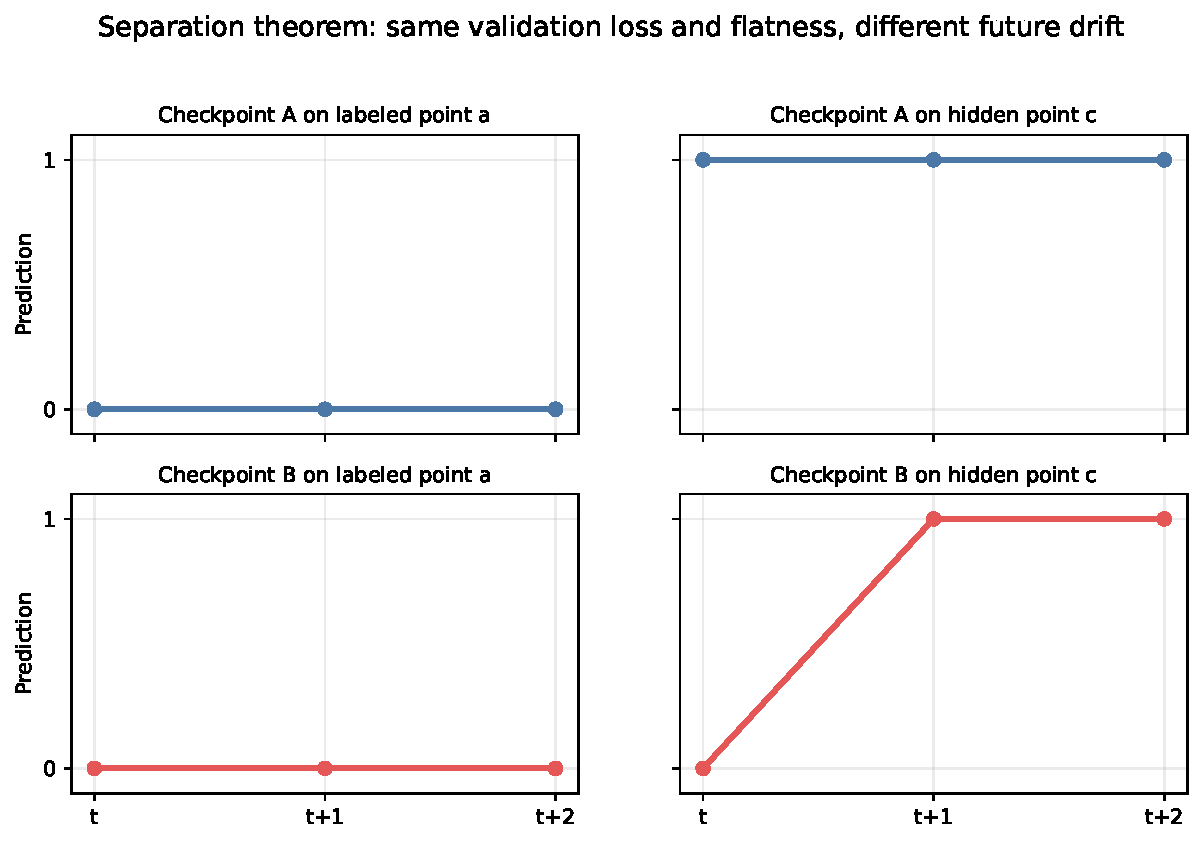
\includegraphics[width=\linewidth]{figures/separation_toy_timeline.pdf}
    \caption{\textbf{Separation theorem intuition.} Two checkpoints can have the same labeled-validation loss and the same local flatness, yet one still contains a hidden support point whose prediction is being renegotiated by SGD. \stawa{} sees that hidden instability through future drift; a flatness-only selector does not.}
    \label{fig:separation}
\end{figure}

\subsection{Dense checkpointing and low-drift averaging}

\begin{proposition}[Dense checkpoint selection converges to the continuous optimum]
\label{prop:dense}
Let $\theta:[0,T]\to\RR^p$ be a continuous training trajectory and let $s(t)$ be an $L_s$-Lipschitz score along the trajectory. Suppose checkpoints are saved at times $0=t_1<\cdots<t_K=T$ with maximum gap $\Delta=\max_k (t_{k+1}-t_k)$. Then
\begin{equation}
    \min_{1\le k\le K} s(t_k)
    \le
    \min_{t\in[0,T]} s(t) + \frac{L_s\Delta}{2}.
\end{equation}
\end{proposition}

\begin{proposition}[Weight averaging is safe under local prediction linearity]
\label{prop:avg}
Assume:
\begin{enumerate}[label=(\roman*), leftmargin=1.5em]
    \item for every input $x$, the map $\theta \mapsto p_\theta(x)$ is twice differentiable on a convex neighborhood containing the selected window,
    \item $\norm{\nabla_\theta^2 p_\theta(x)}_{\mathrm{op}} \le M_p$ on that neighborhood, and
    \item $\ell(y,p)$ is convex in $p$ and $L_d$-Lipschitz with respect to the prediction norm.
\end{enumerate}
Let $\theta_W = \sum_{t\in W} w_t \theta_t$ with convex weights $\{w_t\}_{t\in W}$. Then for any distribution $Q$,
\begin{equation}
    R_Q(\theta_W)
    \le
    \sum_{t\in W} w_t R_Q(\theta_t)
    +
    \frac{L_d M_p}{2}
    \sum_{t\in W} w_t \norm{\theta_t-\theta_W}_2^2.
    \label{eq:avg_bound}
\end{equation}
\end{proposition}

Proposition~\ref{prop:avg} is the local regularity statement needed to justify the final averaging step: if the selected window lies in a low-diameter locally linear region, weight averaging behaves like safe prediction averaging up to a controlled second-order remainder.

\section{Experimental Protocol}
\label{sec:experiments}

This manuscript is complete as a method and theory paper draft, but all \stawa{}-specific experiments remain unrun. The sections below therefore specify the full evaluation protocol and the exact published numbers to beat.

\subsection{Benchmarks and backbone}

We will evaluate on the five standard DomainBed datasets used by \swad{} and DiWA: PACS \citep{li2017pacs}, VLCS \citep{fang2013vlcs}, OfficeHome \citep{venkateswara2017officehome}, TerraIncognita \citep{beery2018terraincognita}, and DomainNet \citep{peng2019domainnet}. Following prior work \citep{cha2021wad,rame2022diwa,gulrajani2021in}, the primary backbone is ResNet-50 and the primary protocol is leave-one-domain-out evaluation with model selection on held-out source validation data.

\subsection{Baselines}

We will compare against:
\begin{itemize}[leftmargin=1.4em]
    \item ERM \citep{gulrajani2021in},
    \item CORAL \citep{sun2016coral},
    \item SWA \citep{izmailov2018swa},
    \item \swad{} \citep{cha2021wad},
    \item DiWA \citep{rame2022diwa},
    \item best validation checkpoint / early stopping,
    \item last checkpoint,
    \item EMA / moving-average checkpointing,
    \item lowest adjacent-drift checkpoint,
    \item latest plateau checkpoint,
    \item optional auxiliary comparisons to prediction-only checkpoint ensembles \citep{chen2017checkpoint}.
\end{itemize}

\subsection{\stawa{} variants}

The planned variants are:
\begin{itemize}[leftmargin=1.4em]
    \item \textbf{\stawa-Mean}: $L_V + \lambda_1 \mu$,
    \item \textbf{\stawa-MeanVar}: $L_V + \lambda_1 \mu + \lambda_2 \sigma$ (default),
    \item \textbf{\stawa-Tail}: replace $\sigma$ by an empirical top-quantile or CVaR drift term,
    \item \textbf{\stawa-Single}: best single checkpoint,
    \item \textbf{\stawa-Window}: contiguous low-score averaging around the best global selector score (default).
\end{itemize}

We will also compare divergence choices:
\begin{itemize}[leftmargin=1.4em]
    \item total variation / $\ell_1$,
    \item Jensen--Shannon divergence,
    \item KL divergence,
    \item squared prediction difference for regression-style tasks.
\end{itemize}

\subsection{Key falsifiable plots}

Three figures are decisive for this paper:
\begin{enumerate}[leftmargin=1.4em]
    \item checkpoint future drift versus final \ood{} accuracy correlation,
    \item pairs of checkpoints with similar loss/flatness but different drift,
    \item ablations showing that low drift is not just ``later checkpoints,'' adjacent smoothness, or early stopping in disguise.
\end{enumerate}

\begin{figure}[t]
    \centering
    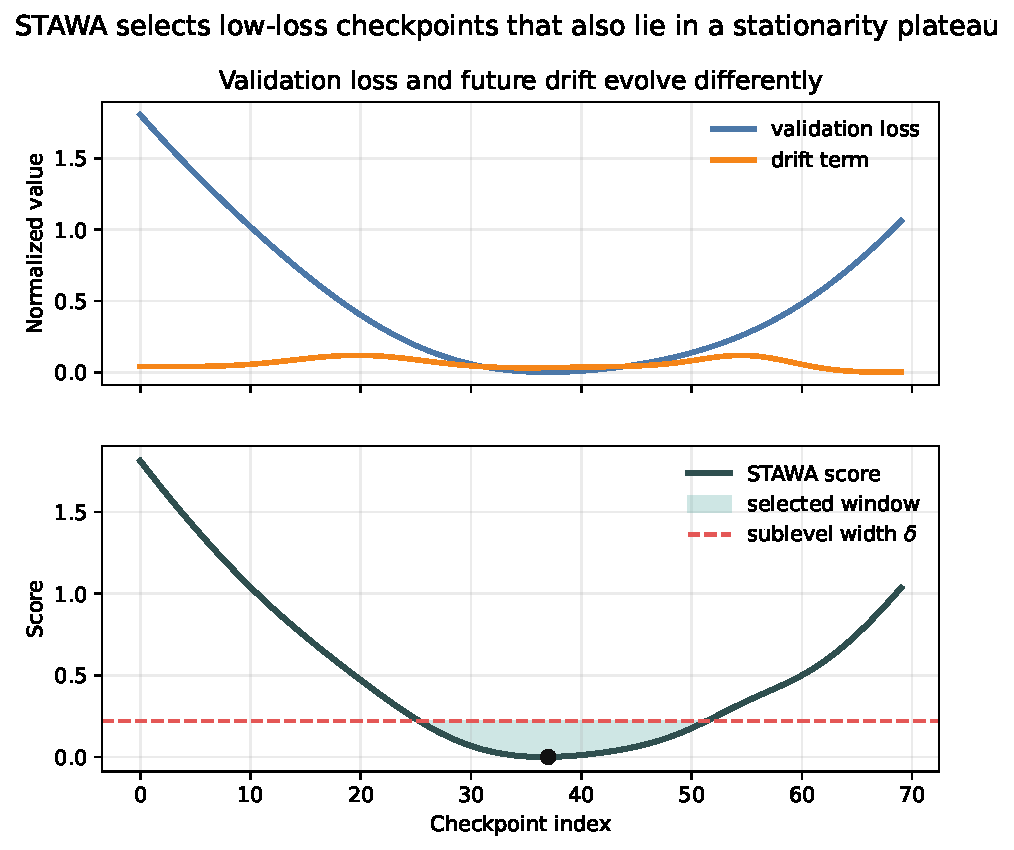
\includegraphics[width=\linewidth]{figures/drift_window_schematic.pdf}
    \caption{\textbf{Dense checkpointing and low-score window selection.} \stawa{} preserves the same practical scaffold that made \swad{} attractive: dense checkpointing and averaging within one connected low-score region. The difference is that the selector targets functional stationarity rather than parameter-space flatness.}
    \label{fig:window}
\end{figure}

\section{Published Reference Results and Placeholder Tables}
\label{sec:results}

We include exact published baselines from prior work so that the empirical target is explicit before running \stawa{}. Every new \stawa{} row remains intentionally marked as \TBD{}.

\begin{table*}[t]
    \centering
    \small
    \setlength{\tabcolsep}{5pt}
    \caption{\textbf{Published reference results on DomainBed with ResNet-50.} Numbers are copied from the cited papers and included here as reference targets for the planned \stawa{} evaluation.}
    \label{tab:published}
    \begin{tabular}{lcccccc}
        \toprule
        Method & PACS & VLCS & OfficeHome & TerraInc & DomainNet & Avg \\
        \midrule
        ERM \citep{cha2021wad,rame2022diwa} & 85.5 & 77.5 & 66.5 & 46.1 & 40.9 & 63.3 \\
        CORAL \citep{rame2022diwa} & 86.2 & 78.8 & 68.7 & 47.6 & 41.5 & 64.6 \\
        \swad{} \citep{cha2021wad} & 88.1 & 79.1 & 70.6 & 50.0 & 46.5 & 66.9 \\
        CORAL + \swad{} \citep{cha2021wad} & 88.3 & 78.9 & 71.3 & 51.0 & 46.8 & 67.3 \\
        DiWA (random init, $M=60$) \citep{rame2022diwa} & 89.0 & 79.4 & 71.6 & 49.0 & 46.3 & 67.1 \\
        DiWA (LP init, $M=60$) \citep{rame2022diwa} & 89.0 & 78.6 & 72.8 & 51.9 & 47.7 & 68.0 \\
        \midrule
        \stawa-Mean (ours) & \TBD & \TBD & \TBD & \TBD & \TBD & \TBD \\
        \stawa-MeanVar (ours) & \TBD & \TBD & \TBD & \TBD & \TBD & \TBD \\
        \stawa-Tail (ours) & \TBD & \TBD & \TBD & \TBD & \TBD & \TBD \\
        \bottomrule
    \end{tabular}
\end{table*}

\begin{table}[t]
    \centering
    \small
    \setlength{\tabcolsep}{3.0pt}
    \renewcommand{\arraystretch}{1.15}
    \caption{\textbf{Published \swad{} ablations copied from \citet{cha2021wad}.} These results motivate dense checkpointing and contiguous window averaging, which \stawa{} preserves.}
    \label{tab:swad_ablation}
    \adjustbox{max width=\linewidth}{
    \begin{tabular}{@{}l|cccc|ccc|ccc@{}}
        \toprule
        & \multicolumn{4}{c|}{Configuration} & \multicolumn{3}{c|}{Out-of-domain} & \multicolumn{3}{c}{In-domain} \\
        & $t_s$ & $t_e$ & lr & interval & PACS & VLCS & Avg. & PACS & VLCS & Avg. \\
        \midrule
        SWA$_{\text{w/ cyclic}}$ & 4000 & 5000 & Cyclic & 100 & 85.9 $\pm 0.1$ & 76.6 $\pm 0.1$ & 81.2 & 97.1 $\pm 0.1$ & 85.0 $\pm 0.2$ & 91.0 \\
        SWA$_{\text{w/ const}}$ & 4000 & 5000 & Const & 100 & 86.5 $\pm 0.3$ & 76.7 $\pm 0.2$ & 81.6 & 97.3 $\pm 0.1$ & 85.0 $\pm 0.2$ & 91.1 \\
        SWAD$_{\text{w/o Dense}}$ & Opt & Overfit & Const & 100 & 86.5 $\pm 0.4$ & 78.0 $\pm 0.7$ & 82.2 & 97.6 $\pm 0.1$ & 85.8 $\pm 0.4$ & 91.7 \\
        SWAD$_{\text{w/o Opt-Overfit}}$ & 4000 & 5000 & Const & 1 & 86.6 $\pm 0.6$ & 76.9 $\pm 0.3$ & 81.7 & 97.5 $\pm 0.1$ & 85.2 $\pm 0.1$ & 91.3 \\
        SWAD$_{\text{w/o Overfit}}$ & Opt & 5000 & Const & 1 & 87.1 $\pm 0.3$ & 77.6 $\pm 0.1$ & 82.4 & 97.7 $\pm 0.1$ & 85.8 $\pm 0.3$ & 91.8 \\
        SWAD$_{\text{fit-on-val}}$ & Val & Val & Const & 1 & 86.2 $\pm 0.2$ & 78.6 $\pm 0.1$ & 82.4 & 97.5 $\pm 0.2$ & 85.8 $\pm 0.3$ & 91.7 \\
        SWAD (proposed) & Opt & Overfit & Const & 1 & 87.1 $\pm 0.2$ & 78.9 $\pm 0.2$ & 83.0 & 97.7 $\pm 0.1$ & 86.1 $\pm 0.5$ & 91.9 \\
        \bottomrule
    \end{tabular}
    }
\end{table}

\begin{table*}[t]
    \centering
    \small
    \caption{\textbf{Planned main results table.} Every \stawa{} cell remains intentionally left as \TBD{} pending experiments.}
    \label{tab:main_tbd}
    \begin{tabular}{lcccccc}
        \toprule
        Method & PACS & VLCS & OfficeHome & TerraInc & DomainNet & Avg \\
        \midrule
        \swad{} & 88.1 & 79.1 & 70.6 & 50.0 & 46.5 & 66.9 \\
        DiWA (best published) & 89.0 & 78.6 & 72.8 & 51.9 & 47.7 & 68.0 \\
        \stawa-Mean & \TBD & \TBD & \TBD & \TBD & \TBD & \TBD \\
        \stawa-MeanVar & \TBD & \TBD & \TBD & \TBD & \TBD & \TBD \\
        \stawa-Tail & \TBD & \TBD & \TBD & \TBD & \TBD & \TBD \\
        \bottomrule
    \end{tabular}
\end{table*}

\begin{table}[t]
    \centering
    \small
    \caption{\textbf{Planned \stawa{} ablations.} These rows are intentionally blank pending experiments.}
    \label{tab:ablations}
    \begin{tabular}{lc}
        \toprule
        Ablation & Avg \\
        \midrule
        Mean only vs. mean + variance & \TBD \\
        Mean + variance vs. CVaR tail term & \TBD \\
        TV vs. JS vs. KL drift & \TBD \\
        Single checkpoint vs. contiguous low-score window & \TBD \\
        Horizon length $H$ & \TBD \\
        Best-val / last / EMA / adjacent-drift / latest-plateau baselines & \TBD \\
        Drift/\ood{} correlation & \TBD \\
        Compute overhead vs. \swad{} & \TBD \\
        \bottomrule
    \end{tabular}
\end{table}

\section{Discussion and Limitations}

\paragraph{What the theory proves.}
The theory proves six concrete points. First, mean predictive drift controls the risk gap between a checkpoint and its local prediction plateau. Second, the variance term controls hidden unstable subsets and bounded density-ratio shifts. Third, the empirical validation and stationarity components concentrate uniformly over dense checkpoint sequences. Fourth, finite samples recover global-score ranking whenever the population margins are large enough. Fifth, the target-risk certificate depends on validation fit, mean drift, and drift spread as the controllable terms. Sixth, flatness-only selectors can be provably blind on an explicit class of examples.

\paragraph{What the theory does not prove.}
The theory does not prove universal empirical superiority over \swad{}, DiWA, or any other DG method. It cannot. It also does not prove that every low-drift checkpoint is semantically robust. The value of the theory is narrower and more honest: it identifies a failure mode of flatness-only selection, gives a measurable function-space alternative, and shows why that alternative is a principled selector inside one completed trajectory.

\paragraph{The main practical risk.}
Low future drift is not automatically the same as good \ood{} generalization. A predictor can be stably wrong. The paper's empirical burden is therefore clear: it must show that functionally stationary checkpoints correlate with \ood{} quality more strongly than flatness-only signals do.

\paragraph{The main competing explanation.}
The most serious hostile-review interpretation is that \stawa{} merely rediscovers late-phase checkpoint selection. That is exactly why the baseline suite must include best validation, last checkpoint, EMA, adjacent-drift selection, and latest-plateau heuristics. If those simpler timing rules explain the same gains, then \stawa{} is not yet a new DG signal.

\paragraph{Why the future-looking stationarity score is still acceptable.}
\stawa{} is explicitly a post-hoc trajectory selector. Its stationarity score depends on future checkpoints inside one completed run. That is not a bug in this setting; it is the defining object. The method would only become problematic if it were sold as an online training rule, which this paper does not do.

\paragraph{Current limitation of this manuscript.}
The obvious limitation is empirical: the \stawa{} experiments have not yet been run. The manuscript is therefore complete as a theory-and-method paper draft, but not complete as a submission-ready empirical claim until the \TBD{} sections are filled.

\section{Conclusion}

We proposed STAWA-Old, a label-free single-run retrospective DG selector based on functional stationarity rather than pooled flatness. The method scores every checkpoint by source validation loss plus mean and spread of short-horizon predictive drift, then averages a contiguous low-score window around the best checkpoint. Our analysis shows that low drift places a checkpoint near its local plateau, that variance controls hidden unstable subsets, that the empirical components concentrate and recover global-score ranking, and that flatness-only selectors can miss target-relevant instability that \stawa{} captures. The empirical results remain to be run, but the manuscript now contains the method, the theory, the figures, the protocol, and the published baselines needed to test whether functional stationarity is a genuinely new selector principle rather than a repackaging of late-phase checkpoint smoothing.

\bibliographystyle{unsrtnat}
\bibliography{references}

\appendix

\section{Detailed Proofs}

\subsection{Proof of Theorem~\ref{thm:plateau}}

\begin{proof}
We first prove Eq.~\eqref{eq:plateau_bound}. Fix an input $x$. By definition,
\begin{equation}
    \bar p_{t,H}(x) - p_t(x)
    =
    \frac{1}{H+1}\sum_{h=1}^{H}\left(p_{t+h}(x)-p_t(x)\right).
\end{equation}
Since $d$ is induced by a norm, the triangle inequality gives
\begin{align}
    d\!\left(p_t(x), \bar p_{t,H}(x)\right)
    &=
    \left\|
    \frac{1}{H+1}\sum_{h=1}^{H}\left(p_{t+h}(x)-p_t(x)\right)
    \right\| \\
    &\le
    \frac{1}{H+1}\sum_{h=1}^{H} d\!\left(p_t(x), p_{t+h}(x)\right) \\
    &\le
    \frac{1}{H}\sum_{h=1}^{H} d\!\left(p_t(x), p_{t+h}(x)\right)
    =
    \Delta_t(x).
\end{align}
By Assumption~\ref{ass:lipschitz},
\begin{equation}
    \ell\!\left(y, p_t(x)\right)
    \le
    \ell\!\left(y, \bar p_{t,H}(x)\right)
    +
    L_d \Delta_t(x).
\end{equation}
Taking expectation over $(x,y)\sim Q$ yields
\begin{equation}
    R_Q(p_t)
    \le
    R_Q(\bar p_{t,H}) + L_d \mu_t^Q.
\end{equation}
This proves Eq.~\eqref{eq:plateau_bound}.

For Eq.~\eqref{eq:plateau_jensen}, fix $(x,y)$. By convexity of $\ell(y,\cdot)$,
\begin{equation}
    \ell\!\left(y,\bar p_{t,H}(x)\right)
    =
    \ell\!\left(
        y,
        \frac{1}{H+1}\sum_{h=0}^{H} p_{t+h}(x)
    \right)
    \le
    \frac{1}{H+1}\sum_{h=0}^{H}\ell\!\left(y,p_{t+h}(x)\right).
\end{equation}
Taking expectation over $(x,y)\sim Q$ proves
\begin{equation}
    R_Q(\bar p_{t,H})
    \le
    \frac{1}{H+1}\sum_{h=0}^{H} R_Q(p_{t+h}).
\end{equation}
\end{proof}

\subsection{Proof of Theorem~\ref{thm:subset}}

\begin{proof}
Let $I_A$ denote the indicator of the subset $A$. Since $P(A)=\rho$,
\begin{equation}
    \EE[\Delta \mid A]
    =
    \frac{\EE[\Delta I_A]}{\rho}.
\end{equation}
Now decompose
\begin{align}
    \EE[\Delta I_A]
    &=
    \EE[\Delta]\EE[I_A]
    +
    \operatorname{Cov}(\Delta, I_A) \\
    &=
    \rho \mu + \operatorname{Cov}(\Delta, I_A).
\end{align}
By Cauchy--Schwarz,
\begin{equation}
    \operatorname{Cov}(\Delta, I_A)
    \le
    \sqrt{\operatorname{Var}(\Delta)\operatorname{Var}(I_A)}
    =
    \sigma \sqrt{\rho(1-\rho)}.
\end{equation}
Therefore
\begin{equation}
    \EE[\Delta I_A]
    \le
    \rho \mu + \sigma \sqrt{\rho(1-\rho)}.
\end{equation}
Dividing by $\rho$ gives
\begin{equation}
    \EE[\Delta \mid A]
    \le
    \mu + \sigma \sqrt{\frac{1-\rho}{\rho}}.
\end{equation}
\end{proof}

\subsection{Proof of Corollary~\ref{cor:density}}

\begin{proof}
Let
\begin{equation}
    w(x) \triangleq \frac{dP_T}{dP_U}(x).
\end{equation}
Then $w\ge 0$, $\EE_{P_U}[w]=1$, and $w\le 1/\rho$ almost surely. The target drift can be written as
\begin{equation}
    \mu_t^T
    =
    \EE_{P_T}[\Delta_t(x)]
    =
    \EE_{P_U}[w(x)\Delta_t(x)].
\end{equation}
Decompose
\begin{align}
    \EE_{P_U}[w\Delta_t]
    &=
    \EE_{P_U}[w]\EE_{P_U}[\Delta_t]
    +
    \operatorname{Cov}_{P_U}(w,\Delta_t) \\
    &=
    \mu_t^U + \operatorname{Cov}_{P_U}(w,\Delta_t).
\end{align}
Again by Cauchy--Schwarz,
\begin{equation}
    \operatorname{Cov}_{P_U}(w,\Delta_t)
    \le
    \sqrt{\operatorname{Var}_{P_U}(w)}\, \sigma_t^U.
\end{equation}
It remains to bound the variance of $w$. Since $0\le w\le 1/\rho$ and $\EE[w]=1$,
\begin{equation}
    \EE[w^2]
    \le
    \frac{1}{\rho}\EE[w]
    =
    \frac{1}{\rho}.
\end{equation}
Therefore
\begin{equation}
    \operatorname{Var}(w)
    =
    \EE[w^2]-\EE[w]^2
    \le
    \frac{1}{\rho}-1
    =
    \frac{1-\rho}{\rho}.
\end{equation}
Combining the last two displays yields
\begin{equation}
    \mu_t^T
    \le
    \mu_t^U + \sigma_t^U \sqrt{\frac{1-\rho}{\rho}}.
\end{equation}
\end{proof}

\subsection{Proof of Proposition~\ref{prop:concentration}}

\begin{proof}
The validation loss is bounded in $[0,1]$, so Hoeffding's inequality gives, for each $t$,
\begin{equation}
    \Pr\!\left(
        \left| \hat L_V(\theta_t)-R_V(p_t) \right| > \epsilon
    \right)
    \le
    2e^{-2n\epsilon^2}.
\end{equation}
Applying a union bound over $t=1,\dots,K-H$ proves Eq.~\eqref{eq:conc_loss}.

Next, each drift variable $\Delta_t(x_i)$ lies in $[0,1]$, so another application of Hoeffding plus a union bound gives Eq.~\eqref{eq:conc_mu}.

For the standard deviation term, define
\begin{equation}
    m_{2,t} \triangleq \EE[(\Delta_t)^2],
    \qquad
    \hat m_{2,t} \triangleq \frac{1}{m}\sum_{i=1}^{m}\Delta_t(x_i)^2.
\end{equation}
Since $\Delta_t(x_i)^2\in[0,1]$, Hoeffding and a union bound yield
\begin{equation}
    |\hat m_{2,t}-m_{2,t}|
    \le
    \sqrt{\frac{\log(8(K-H)/\delta)}{2m}}
\end{equation}
simultaneously for all $t$ with probability at least $1-\delta/2$.

Now
\begin{equation}
    \sigma_t^2 = m_{2,t} - (\mu_t^U)^2,
    \qquad
    \hat \sigma_t^2 = \hat m_{2,t} - (\hat \mu_t)^2.
\end{equation}
Hence
\begin{align}
    |\hat \sigma_t^2 - \sigma_t^2|
    &\le
    |\hat m_{2,t}-m_{2,t}| + |(\hat \mu_t)^2-(\mu_t^U)^2| \\
    &\le
    |\hat m_{2,t}-m_{2,t}| + |\hat \mu_t-\mu_t^U|\,|\hat \mu_t+\mu_t^U| \\
    &\le
    |\hat m_{2,t}-m_{2,t}| + 2|\hat \mu_t-\mu_t^U|,
\end{align}
because both means lie in $[0,1]$. Using the previous bounds gives
\begin{equation}
    |\hat \sigma_t^2 - \sigma_t^2|
    \le
    3\sqrt{\frac{\log(8(K-H)/\delta)}{2m}}.
\end{equation}
Finally, since $u\mapsto \sqrt{u}$ is $1/2$-H\"older on $[0,\infty)$,
\begin{equation}
    |\hat \sigma_t - \sigma_t|
    \le
    \sqrt{|\hat \sigma_t^2 - \sigma_t^2|}
    \le
    \sqrt{
        3\sqrt{\frac{\log(8(K-H)/\delta)}{2m}}
    }.
\end{equation}
Combining the bounds on $\hat\mu_t$ and $\hat\sigma_t$ proves Eq.~\eqref{eq:conc_j}; Eq.~\eqref{eq:conc_loss} is already the validation-loss component bound needed for the global score.
\end{proof}

\subsection{Proof of Proposition~\ref{prop:plateau_membership}}

\begin{proof}
By Proposition~\ref{prop:concentration}, with probability at least $1-\delta$ we have simultaneously
\begin{equation}
    |\hat L_V(\theta_u)-R_V(p_u)|
    \le
    \eta_{n,\delta}
    \qquad
    \text{for every } u\in\{1,\dots,K-H\}.
\end{equation}
Fix that event. Let $u^\star$ be a minimizer of $R_V(p_u)$, so $R_V(p_{u^\star})=L_V^\star$. Then
\begin{equation}
    \hat L_V^\star
    \le
    \hat L_V(\theta_{u^\star})
    \le
    L_V^\star + \eta_{n,\delta}.
\end{equation}
Now suppose
\begin{equation}
    R_V(p_t) \le L_V^\star + \epsilon - 2\eta_{n,\delta}.
\end{equation}
Then
\begin{equation}
    \hat L_V(\theta_t)
    \le
    R_V(p_t) + \eta_{n,\delta}
    \le
    L_V^\star + \epsilon - \eta_{n,\delta}
    \le
    \hat L_V^\star + \epsilon,
\end{equation}
so $t\in\widehat{\mathcal{A}}_{\epsilon}$.

Conversely, if
\begin{equation}
    R_V(p_t) \ge L_V^\star + \epsilon + 2\eta_{n,\delta},
\end{equation}
then
\begin{equation}
    \hat L_V(\theta_t)
    \ge
    R_V(p_t) - \eta_{n,\delta}
    \ge
    L_V^\star + \epsilon + \eta_{n,\delta}
    \ge
    \hat L_V^\star + \epsilon,
\end{equation}
so $t\notin\widehat{\mathcal{A}}_{\epsilon}$. This proves both implications.
\end{proof}

\subsection{Proof of Corollary~\ref{cor:ranking}}

\begin{proof}
By Proposition~\ref{prop:concentration}, with probability at least $1-\delta$ we have simultaneously
\begin{equation}
    |\hat J_u - J_u^\star|
    \le
    \eta_{J,m,\delta}
    \qquad
    \text{for every } u\in\{1,\dots,K-H\}.
\end{equation}
On the same event, Proposition~\ref{prop:plateau_membership} implies that every checkpoint in $\mathcal{A}_{\epsilon-2\eta_{n,\delta}}^\star$ belongs to $\widehat{\mathcal{A}}_{\epsilon}$. Hence $s,t\in\widehat{\mathcal{A}}_{\epsilon}$.

Finally,
\begin{equation}
    \hat J_s
    \le
    J_s^\star + \eta_{J,m,\delta}
    <
    J_t^\star - \eta_{J,m,\delta}
    \le
    \hat J_t,
\end{equation}
where the strict middle inequality uses the assumed population margin
\begin{equation}
    J_s^\star + 2\eta_{J,m,\delta} < J_t^\star.
\end{equation}
Therefore $\hat J_s < \hat J_t$ with probability at least $1-\delta$.
\end{proof}

\subsection{Proof of Theorem~\ref{thm:certificate}}

\begin{proof}
By Theorem~\ref{thm:plateau},
\begin{equation}
    R_T(p_t)
    \le
    R_T(\bar p_{t,H}) + L_d \mu_t^T.
    \label{eq:cert_1}
\end{equation}
By definition of $\Gamma_t$,
\begin{equation}
    R_T(\bar p_{t,H})
    \le
    R_V(\bar p_{t,H}) + \Gamma_t.
    \label{eq:cert_2}
\end{equation}
Applying Theorem~\ref{thm:plateau} again, now on the source distribution $V$,
\begin{equation}
    R_V(\bar p_{t,H})
    \le
    R_V(p_t) + L_d \mu_t^S.
    \label{eq:cert_3}
\end{equation}
Combining Eqs.~\eqref{eq:cert_1}--\eqref{eq:cert_3} gives
\begin{equation}
    R_T(p_t)
    \le
    R_V(p_t) + \Gamma_t + L_d(\mu_t^S+\mu_t^T).
    \label{eq:cert_4}
\end{equation}
By Corollary~\ref{cor:density},
\begin{equation}
    \mu_t^T
    \le
    \mu_t^S + \sigma_t^S \sqrt{\frac{1-\rho}{\rho}}.
\end{equation}
Substituting this into Eq.~\eqref{eq:cert_4} yields
\begin{equation}
    R_T(p_t)
    \le
    R_V(p_t)
    +
    \Gamma_t
    +
    L_d\left(
        2\mu_t^S + \sigma_t^S \sqrt{\frac{1-\rho}{\rho}}
    \right).
\end{equation}
Finally, because the validation loss is bounded in $[0,1]$, Hoeffding's inequality with a union bound over $t=1,\dots,K-H$ gives
\begin{equation}
    R_V(p_t)
    \le
    \hat R_V(p_t) + \sqrt{\frac{\log(2(K-H)/\delta)}{2n}}
\end{equation}
simultaneously for all $t$ with probability at least $1-\delta$. Combining the last two displays proves Eq.~\eqref{eq:certificate}.
\end{proof}

\subsection{Proof of Theorem~\ref{thm:separation}}

\begin{proof}
Part (i) is immediate. The labeled validation set contains only the point $a$ with label $0$, and both checkpoints predict $0$ on that point. Therefore
\begin{equation}
    L_V(\theta_A)=L_V(\theta_B)=0.
\end{equation}
By construction, the local labeled-validation loss landscapes are identical quadratic functions, so any local flatness statistic computed from them is also identical.

For part (ii), checkpoint $A$ is perfectly stationary over the one-step horizon on both support points:
\begin{equation}
    \Delta_A(a)=|p_A(a)-p_{A^+}(a)|=0,
    \qquad
    \Delta_A(c)=|p_A(c)-p_{A^+}(c)|=0.
\end{equation}
Hence $\mu_A=0$ and $\sigma_A=0$.

Checkpoint $B$ is stationary on $a$ but not on $c$:
\begin{equation}
    \Delta_B(a)=|0-0|=0,
    \qquad
    \Delta_B(c)=|0-1|=1.
\end{equation}
Since $U$ is uniform on $\{a,c\}$,
\begin{equation}
    \mu_B = \frac{0+1}{2}=\frac{1}{2}.
\end{equation}
The variance is
\begin{equation}
    \sigma_B^2
    =
    \frac{1}{2}\left(0-\frac{1}{2}\right)^2 + \frac{1}{2}\left(1-\frac{1}{2}\right)^2
    =
    \frac{1}{4},
\end{equation}
so $\sigma_B=\frac{1}{2}$. Therefore
\begin{equation}
    S_B-S_A
    =
    \lambda_1\left(\frac{1}{2}\right)+\lambda_2\left(\frac{1}{2}\right)
    =
    \frac{\lambda_1+\lambda_2}{2}
    >
    0.
\end{equation}

For part (iii), the target distribution is concentrated on $c$ with label $1$. Under squared loss,
\begin{equation}
    R_T(p_A) = (1-1)^2 = 0,
    \qquad
    R_T(p_B) = (0-1)^2 = 1.
\end{equation}
This proves the strict target-risk separation.
\end{proof}

\subsection{Proof of Proposition~\ref{prop:dense}}

\begin{proof}
Let $t^\star\in\argmin_{t\in[0,T]} s(t)$. By construction of the grid, there exists some checkpoint time $t_k$ satisfying $|t_k-t^\star|\le \Delta/2$. Since $s$ is $L_s$-Lipschitz,
\begin{equation}
    s(t_k)
    \le
    s(t^\star) + L_s|t_k-t^\star|
    \le
    s(t^\star) + \frac{L_s\Delta}{2}.
\end{equation}
Taking the minimum over $k$ proves the claim.
\end{proof}

\subsection{Proof of Proposition~\ref{prop:avg}}

\begin{proof}
Let
\begin{equation}
    \bar p_W(x) \triangleq \sum_{t\in W} w_t p_{\theta_t}(x)
\end{equation}
be the prediction-space average over the selected window, and let
\begin{equation}
    \theta_W \triangleq \sum_{t\in W} w_t \theta_t.
\end{equation}
Fix an input $x$. By Taylor's theorem around $\theta_W$, for each $t\in W$ there exists a point $\xi_t(x)$ on the segment between $\theta_W$ and $\theta_t$ such that
\begin{equation}
    p_{\theta_t}(x)
    =
    p_{\theta_W}(x)
    +
    \nabla_\theta p_{\theta_W}(x)^\top (\theta_t-\theta_W)
    +
    \frac{1}{2}(\theta_t-\theta_W)^\top \nabla_\theta^2 p_{\xi_t(x)}(x)(\theta_t-\theta_W).
\end{equation}
Multiply by $w_t$ and sum over $t$. The linear terms cancel because
\begin{equation}
    \sum_{t\in W} w_t (\theta_t-\theta_W) = 0.
\end{equation}
Hence
\begin{equation}
    \bar p_W(x) - p_{\theta_W}(x)
    =
    \frac{1}{2}\sum_{t\in W} w_t
    (\theta_t-\theta_W)^\top \nabla_\theta^2 p_{\xi_t(x)}(x)(\theta_t-\theta_W).
\end{equation}
Taking norms and using the Hessian bound gives
\begin{equation}
    d\!\left(\bar p_W(x), p_{\theta_W}(x)\right)
    \le
    \frac{M_p}{2}\sum_{t\in W} w_t \norm{\theta_t-\theta_W}_2^2.
    \label{eq:avg_local}
\end{equation}
By convexity of $\ell(y,\cdot)$,
\begin{equation}
    \ell\!\left(y,\bar p_W(x)\right)
    \le
    \sum_{t\in W} w_t \ell\!\left(y,p_{\theta_t}(x)\right).
\end{equation}
By $L_d$-Lipschitz continuity,
\begin{equation}
    \ell\!\left(y,p_{\theta_W}(x)\right)
    \le
    \ell\!\left(y,\bar p_W(x)\right)
    +
    L_d\, d\!\left(\bar p_W(x), p_{\theta_W}(x)\right).
\end{equation}
Substituting Eq.~\eqref{eq:avg_local} yields
\begin{equation}
    \ell\!\left(y,p_{\theta_W}(x)\right)
    \le
    \sum_{t\in W} w_t \ell\!\left(y,p_{\theta_t}(x)\right)
    +
    \frac{L_d M_p}{2}
    \sum_{t\in W} w_t \norm{\theta_t-\theta_W}_2^2.
\end{equation}
Taking expectation over $(x,y)\sim Q$ proves Eq.~\eqref{eq:avg_bound}.
\end{proof}

\section{Implementation Notes}

\paragraph{Choice of drift metric.}
The cleanest theory uses a norm-induced discrepancy such as $\ell_1$ or total variation. In practice, Jensen--Shannon or KL drift may correlate better with accuracy for classification. The theory then applies after translating those divergences to total variation through standard inequalities or after clipping probabilities.

\paragraph{Horizon length.}
The horizon $H$ should be long enough to expose unresolved function drift but short enough to stay inside one local training phase. The main paper will treat $H$ as a small hyperparameter and report sensitivity.

\paragraph{Why a contiguous window?}
Contiguity is inherited from SWA and \swad{}. It is not merely aesthetic: it keeps the selected checkpoints inside one local region of the trajectory, which is exactly the regime in which Proposition~\ref{prop:avg} is most credible.

\end{document}
